\documentclass[tikz]{standalone}

\usepackage{tikz}
    \usetikzlibrary{mindmap}

\begin{document}
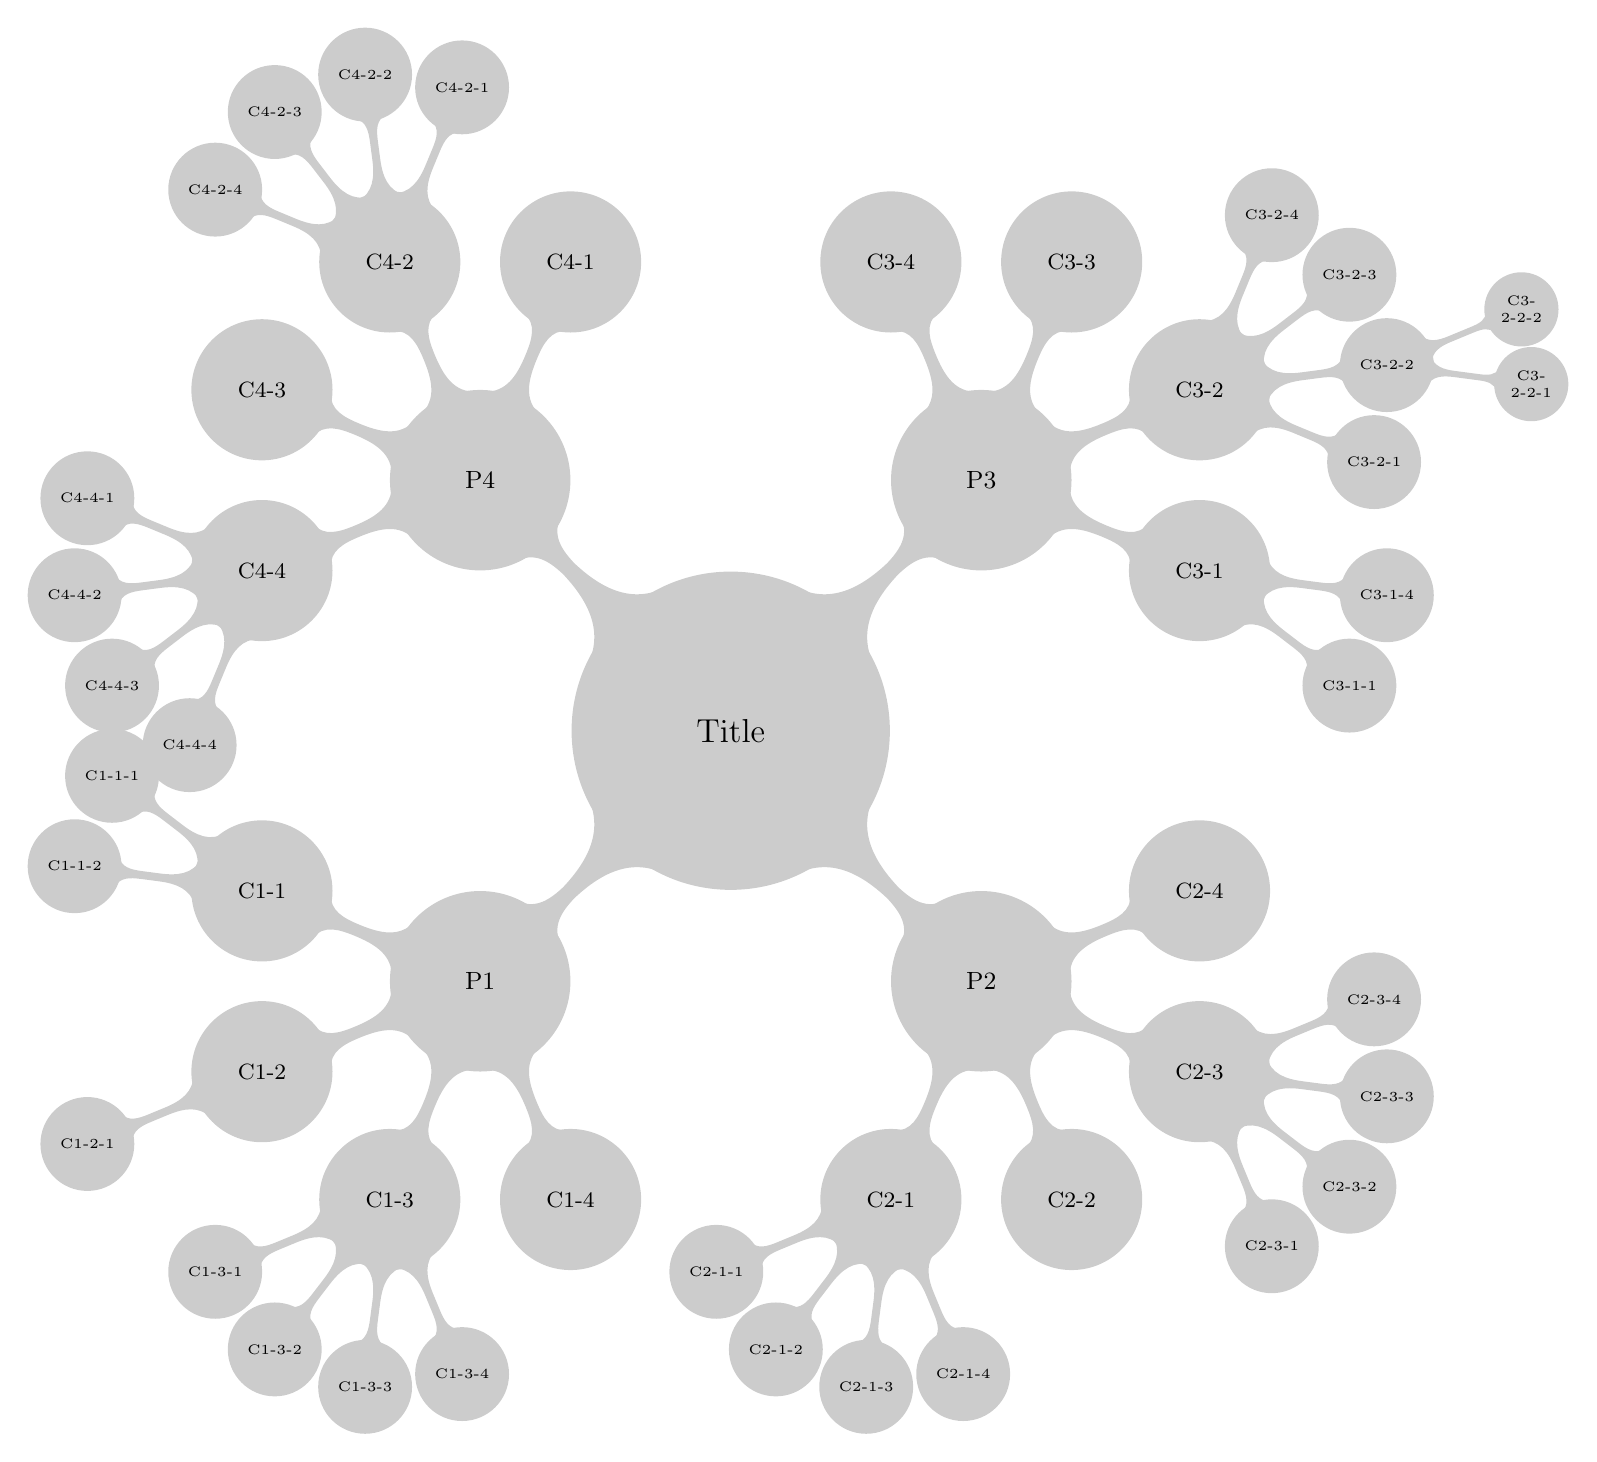
\begin{tikzpicture}[
    mindmap, every node/.style=concept, concept color=black!20,
    grow cyclic,
    level 1/.append style={level distance=4.5cm,sibling angle=90},
    level 2/.append style={level distance=3cm,sibling angle=45}
]

\node (T) {Title} 
    child{ node (1) {P1} 
        child{ node (1-1) {C1-1} 
            child{ node (1-1-1) {C1-1-1} }
            child{ node (1-1-2) {C1-1-2} }}
        child{ node (1-2) {C1-2} 
            child{ node (1-2-1) {C1-2-1} }}
        child{ node (1-3) {C1-3} 
            child{ node (1-3-1) {C1-3-1} }
            child{ node (1-3-2) {C1-3-2} }
            child{ node (1-3-3) {C1-3-3} }
            child{ node (1-3-4) {C1-3-4} }}
        child{ node (1-4) {C1-4} }}
    child{ node (2) {P2} 
        child{ node (2-1) {C2-1} 
            child{ node (2-1-1) {C2-1-1} }
            child{ node (2-1-2) {C2-1-2} }
            child{ node (2-1-3) {C2-1-3} }
            child{ node (2-1-4) {C2-1-4} }}
        child{ node (2-2) {C2-2} }
        child{ node (2-3) {C2-3} 
            child{ node (2-3-1) {C2-3-1} }
            child{ node (2-3-2) {C2-3-2} }
            child{ node (2-3-3) {C2-3-3} }
            child{ node (2-3-4) {C2-3-4} }}
        child{ node (2-4) {C2-4} }}
    child{ node (3) {P3} 
        child{ node (3-1) {C3-1} 
            child{ node (3-1-1) {C3-1-1} }
            child{ node (3-1-2) {C3-1-4} }}
        child{ node (3-2) {C3-2} 
            child{ node (3-2-1) {C3-2-1} }
            child{ node (3-2-2) {C3-2-2} 
                child{ node (3-2-2-1) {C3-2-2-1} }
                child{ node (3-2-2-2) {C3-2-2-2} }}
            child{ node (3-2-3) {C3-2-3} }
            child{ node (3-2-4) {C3-2-4} }}
        child{ node (3-3) {C3-3} }
        child{ node (3-4) {C3-4} }}
    child{ node (4) {P4} 
        child{ node (4-1) {C4-1} }
        child{ node (4-2) {C4-2} 
            child{ node (4-2-1) {C4-2-1} }
            child{ node (4-2-2) {C4-2-2} }
            child{ node (4-2-3) {C4-2-3} }
            child{ node (4-2-4) {C4-2-4} }}
        child{ node (4-3) {C4-3} }
        child{ node (4-4) {C4-4} 
            child{ node (4-4-1) {C4-4-1} }
            child{ node (4-4-2) {C4-4-2} }
            child{ node (4-4-3) {C4-4-3} }
            child{ node (4-4-4) {C4-4-4} }}};

\end{tikzpicture}
\end{document}
